\documentclass{article}
\usepackage{amsmath}
\usepackage{tikz}
\usepackage{pgfplots}
\pgfplotsset{compat=1.18}

\begin{document}

\section*{Toro Parametrization}

\[
S : \begin{cases}
x = (R + r \cos v) \cos u \\
y = (R + r \cos v) \sin u \\
z = r \sin v
\end{cases}
\]

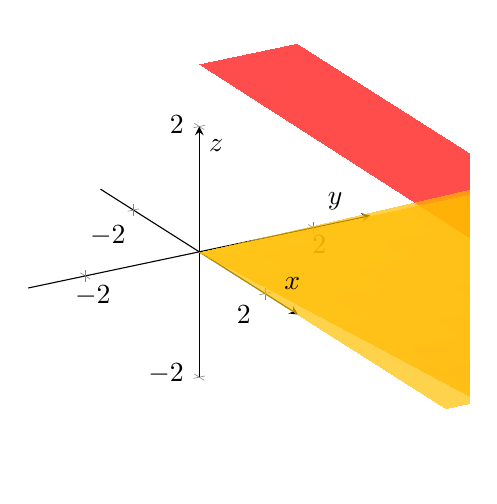
\begin{tikzpicture}
    \begin{axis}[
        axis lines=center,
        xlabel={\(x\)}, ylabel={\(y\)}, zlabel={\(z\)},
        xmin=-3, xmax=3, ymin=-3, ymax=3, zmin=-2, zmax=2,
        grid=major,
        view={60}{30} % Camera angle
    ]
    \addplot3[
        surf,
        shader=interp,
        domain=0:360,
        domain y=0:360,
        samples=40,
        opacity=0.7
    ]
    {(2 + 1*cos(y)) * cos(x)};
    \addplot3[
        surf,
        shader=interp,
        domain=0:360,
        domain y=0:360,
        samples=40,
        opacity=0.7
    ]
    {(2 + 1*cos(y)) * sin(x)};
    \addplot3[
        surf,
        shader=interp,
        domain=0:360,
        domain y=0:360,
        samples=40,
        opacity=0.7
    ]
    {1*sin(y)};
    \end{axis}
\end{tikzpicture}

\end{document}